\subsection{Référentiel et repère}

\begin{UPSTIactivite}
\begin{center}
  \includegraphics[width=.4\textwidth]{Src/Images/bus_mouvement_relatif}
\end{center}

Imaginons qu'une personne $B$ soit dans un bus (voir figure ci-dessus). Elle se déplace de l'avant vers l'arrière du bus. Une personne $A$ est assise dans le train, elle regarde dans le sens de la marche.
\UPSTIquestion{Par rapport à $A$, comment se déplace $B$ ? (Va-t-elle vers l'arrière, vers l'avant ou est-elle immobile ?)}

\UPSTIeleveOnly{\UPSTIpointilles[1]}
\UPSTIcorrection{Pour A, B se déplace vers l'arrière.}
\UPSTIquestion{Pour $A$, cette personne va-t-elle lentement ou rapidement ?}

\UPSTIeleveOnly{\UPSTIpointilles[1]}
\UPSTIcorrection{Pour A, B se déplace lentement.}
\UPSTIquestion{Une personne $C$ est sur le bord de la voie. Elle voit passer le train. Par rapport à $C$, comment se déplace $A$ ? Se déplace-t-elle rapidement ?}

\UPSTIeleveOnly{\UPSTIpointilles[1]}
\UPSTIcorrection{Pour C, B se déplace \textbf{rapidement} vers l'avant.}

\end{UPSTIactivite}

On le voit dans cet exemple, la trajectoire d'un point n'est pas la même selon le point de vue que l'on considère. Ainsi, il est \textbf{impératif} de préciser par rapport à quoi on s'exprime lorsque l'on caractérise un mouvement.

\UPSTIaRetenir{
\begin{itemize}
  \item Afin d'étudier le mouvement d'un point ou d'un système de solides, il est nécessaire de mettre en place un système de référence appelé \textit{référentiel}. Il représente en quelque sorte la position d'observation des phénomènes.
  \item Un repère est défini par une origine $O$ et trois vecteurs orthonormés directs \bxyz. Il se note \rROxyz
  \item La \UPSTIfig{fig:reperes} représente le repère direct \rROxyz vu de différents points de vues.
\end{itemize}
}

\begin{figure}[!ht]
  \centering
  \begin{subfigure}[b]{.3\textwidth}
    \centering
    \dessinRepere[\vx{}][\vy{}][\vz{}][O]
    \caption{\vz{} vers nous}
  \end{subfigure}
  \begin{subfigure}[b]{.3\textwidth}
    \centering
    \dessinRepere[\vz{}][\vx{}][\vy{}][O]
    \caption{\vy{} vers nous}
  \end{subfigure}
  \begin{subfigure}[b]{.3\textwidth}
    \centering
    \dessinRepere[\vy{}][\vz{}][\vx{}][O]
    \caption{\vx{} vers nous}
  \end{subfigure}
  \caption{Le repère \rROxyz}
  \label{fig:reperes}
\end{figure}
\pagebreak


\begin{UPSTIactivite}
  Pour décrire la position d'un point dans un repère, on utilise ses coordonnées par rapport au centre du repère.

    \begin{center}
      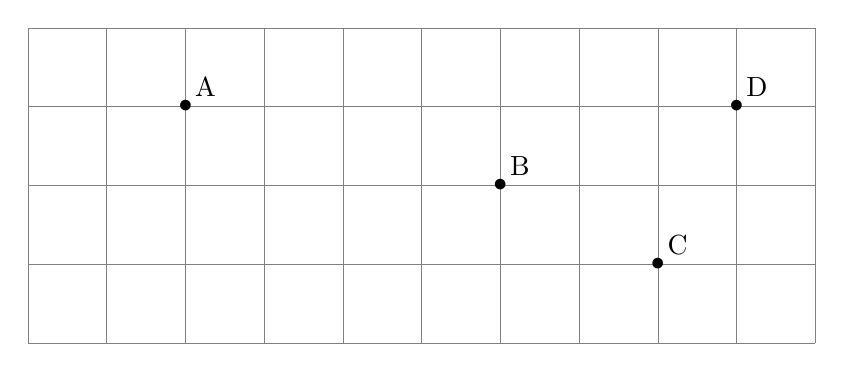
\begin{tikzpicture}
        \draw [very thin, gray] (0,0) grid (10,4);
        \dessinRepereFigGeo[\vx{}][\vy{}][\vz{}][O]
        \begin{scope}[shift={(4,2)}]
          \dessinRepereFigGeo[\vy{1}][\vz{1}][\vx{1}][G]
        \end{scope}
        \draw (2,3) node{$\bullet$} node[above right]{A};
        \draw (6,2) node{$\bullet$} node[above right]{B};
        \draw (8,1) node{$\bullet$} node[above right]{C};
        \UPSTIprofOnly{\draw (9,3) node{$\bullet$} node[above right]{D};}
      \end{tikzpicture}
    \end{center}

    \UPSTIexemple{Le point $C$ a pour coordonnées $(8,1,0)$ dans le repère \rROxyz. Le point $C$ a pour coordonnées $(0,4,-1)$ dans le repère \repere[\rR{1}]{G}{\vx{1}}{\vy{1}}{\vz{1}}.}

  \resetNumQuestion
  % ----- Question ------
  \UPSTIquestion{Donner les coordonnées des points A et B dans le repère \rROxyz}

  \UPSTIeleveOnly{\UPSTIpointilles[1]}

  \UPSTIcorrection{ Dans \rROxyz : $A(2,3,0)$ et $B(6,2,0)$.}

  % ----- Question ------
  \UPSTIquestion{Donner les coordonnées des point A et B dans le repère \repere[\rR{1}]{G}{\vx{1}}{\vy{1}}{\vz{1}} }

  \UPSTIeleveOnly{\UPSTIpointilles[1]}

  \UPSTIcorrection{ Dans \repere[\rR{1}]{G}{\vx{1}}{\vy{1}}{\vz{1}} : $A(0,-2,1)$ et $B(0,2,0)$.}

  \UPSTIquestion{Placer le point $D$ de coordonnées $(0,5,1)$ dans le repère \repere[\rR{1}]{G}{\vx{1}}{\vy{1}}{\vz{1}}}

  \resetNumQuestion
\end{UPSTIactivite}

\subsection{Trajectoire}
\UPSTIdefinition{On appelle trajectoire du point ($M$) d’un solide \solide{S} l’ensemble des positions occupées successivement par ce point, au cours du temps, lors son déplacement par rapport à un référentiel donné. \\
La trajectoire du point $M$ appartenant à \solide{S} par rapport au repère \rR{} se note \trajectoire{M}{S}{R}}

\UPSTIexemple[Trajectoire de la pointe d'un stylo]{
La trajectoire de la pointe du stylo par rapport à la feuille est la trace laissée par cette pointe sur la feuille.

}

\subsubsection{Différents types de trajectoires}
\UPSTIaRetenir{On pourra différentier trois grands types de trajectoires pour un point :

\UPSTIeleveOnly{\UPSTIpointilles}

\UPSTIprofOnly{
  \begin{itemize}
    \item La droite
    \item L'arc de cercle (ou le cercle complet)
    \item Une trajectoire quelconque
  \end{itemize}}
}

\begin{figure}[!ht]
  \centering
  \begin{subfigure}[b]{.3\textwidth}
    \centering
    \begin{tikzpicture}
      \draw (0,0) -- (2,1);
    \end{tikzpicture}
    \caption{Trajectoire droite}
  \end{subfigure}
  \begin{subfigure}[b]{.3\textwidth}
    \centering
    \begin{tikzpicture}
      \draw (1,0) arc (10:170:1) ;
    \end{tikzpicture}
    \caption{Trajectoire circulaire}
  \end{subfigure}
  \begin{subfigure}[b]{.3\textwidth}
    \centering
      \begin{tikzpicture}
        \draw plot [domain=-0.8:0.8] (\x,\x^2);
      \end{tikzpicture}
    \caption{Trajectoire curviligne.}
  \end{subfigure}
  \caption{Différents types de trajectoires.}
  \label{fig:diff_traj}
\end{figure}
